\documentclass[fleqn]{article}

\usepackage[utf8]{inputenc}
\usepackage{cite}

\usepackage{amsfonts}
\usepackage{amsmath}
\usepackage{amssymb}
\usepackage{float}

\usepackage{hyperref}
\usepackage{syntax}
\usepackage{listings}
\usepackage{zed-csp}


\usepackage{tikz}
\usetikzlibrary{positioning}

\lstdefinelanguage{sal}{
  keywords = {send, become, let, new, in, to, if, then, else, case, def, end,
    case, of, ||}
}

\lstdefinelanguage{csp}{
  keywords = {channel, datatype}
}

\lstdefinestyle{simple}{
  basewidth=0.5em
}

\newcommand{\SAL}{\textbf{SAL}}
\newcommand{\CSP}{\textbf{CSP}}
\newcommand{\CSPm}{\textbf{CSPm}}


\title{CSP}
\author{José Luis Diaz}
\date{ }
 
\begin{document}
 
\maketitle
 
\tableofcontents
 
\section{Introducción}

\section{Conceptos básicos}

\subsection{Comportamientos} \label{basicos:comportamientos}

\subsection{Creando Actores}

\subsection{Creando comunicaciones}

\subsection{Comandos}

\section{Lenguaje de Actor Mínimo}

Un programa en \SAL no es mas que una secuencia de \textit{comportamientos}.
Como en la mayoría de los lenguaje de programación, tiene un nombre reservado
\textbf{main}, este \textit{Comportamiento} es el punto de entrada, será el
responsable de crear otros actores y enviar mensajes.

\begin{grammar}
   <Pgm> :== $BDef_1 ... BDef_n BDef_{main} $ 
\end{grammar}

la definición de \textit{comportamientos} funcionan como una suerte de plantilla
para el comportamiento que luego tendrán los actores. 

\subsection{Expresiones}
Existen tres tipos primitivos, booleanos, enteros y dirección del buzón. Las operaciones
posibles entre los booleanos son \textbf{or}, \textbf{and}, \textbf{not}. Con
respecto a los enteros se pueden operar utilizando \textbf{+}, \textbf{-},
\textbf{*}, \textbf{/}. Un buzón es un identificador que es devuelto cuando se
crea un nuevo actor.

\subsection{Definición de comandos}
La gramática de los comandos en SAL es la siguiente:

\begin{grammar}
  <command> ::= `send' $e_1, e_2, \ldots\ , e_n$ `to' <actor>  
  \alt `become' $B(e_1, e_2, ..., e_n)$
  \alt `let' $x_1$ = `new' $B_1(e_1, e_2, ..., e_{1n})$, \\
   \ldots\ \ $x_k$ = `new' $B_k(e_1, e_2, ..., e_{kn})$       \\
  `in' <command> 
  \alt `if`<bool-expr> `then' <command> `else' <command> `end if'
  \alt <command> `||' <command>
\end{grammar}

\begin{description}
\item [send]  Este comando permite enviar mensajes a otros actores, toma como
  parámetro una lista separada por coma de las expresiones a enviar, y el actor
  destino, el envío de mensajes es asincrónico. Cada expresión es evaluada antes
  de ser enviada.
\item [become] Este comando especifica el siguiente comportamiento del actor
  que está procesando la comunicación recibida. Como en el caso anterior se evalúan
  las expresiones antes de ser enviadas, y estas aparecerán como la listas de
  parámetros del comportamiento. 
\item[new] Este comando sirve para crear nuevos actores. El alcance de los
  identificadores de los nuevos actores creados está sujeto al cuerpo de \textbf{let}.
\item[condicional] Luego de evaluar la expresión booleana, si es verdadera
  ejecuta lo que esta a continuación de \textbf{then}, en caso contrario lo que está a
  continuación de \textbf{else}. Funciona como cualquier condicional.
\item[composición] Estos dos comandos en \SAL son ejecutados concurrentemente.
 
\end{description}

La ejecución de los comandos ocurre cuando el actor recibe un mensaje, y todos
ellos ocurren concurrentemente, la composición no es secuencial.

\subsection{Definición de comportamientos}

La sintaxis de los comportamientos es la siguiente:

\begin{grammar}
 <BDef> :== `def' <beh name> `(' <acquaiantence-list> `)' `[`'<input-list>`]' \\
  \quad <command>* \\
  `end def'
  \alt <acquaiantence-list> :== <id> | <id>`,' <acquaiantence-list>
  \alt <input-list> :== <id> | <id>`,' <input-list>
\end{grammar}

El identificador \textit{beh name} esta atado a una abstracción y tiene alcance
a todo el programa. Los identificadores \textit{acquaiantence-list} los recibe el
momento de instanciación y tiene alcance en todo \textit{command}. Los
identificadores \textit{input-list} son completados al momento de recibir un
mensaje, y su alcance es todo \textit{command}. \\
Ambas listas, \textit{input-list} y \textit{acquaiantence-list} contienen todos
los identificadores libres que están en \textit{command}. Existe un
identificador especial \textit{self} que puede ser utilizado para hacer
referencia al actor que está se definiendo. \\
La ejecución de \textit{command} deberá contar a lo sumo con un solo comando
\textit{become}, esta propiedad tiene que ser garantizado de manera estática, de no
existir ningún comando \textit{become}, el actor asumirá un comportamiento de
tipo \textit{bottom}, es es básicamente ignorar los mensajes que se le envíen.

\subsection{Ejemplo}

Está implementación del factorial está adaptada de \cite{Agha:1986:AMC:7929}, esta
depende de un actor \textit{main} que le envía el valor a calcular. El factorial
esta siempre disponible para procesar la siguiente comunicación, no bloquea con
el calculo recursivo del factorial sino que lo delega en otros actores.

La palabra reservada \textit{self} hace referencia a la dirección de buzón
correspondiente al actor que está procesando la comunicación, este es inicializado
cuando el actor es creado.

\begin{lstlisting}[language=sal, style=simple]
def Factorial()[val, customer]
  become factorial() ||
  if val = 0 then
  send [1] to customer
  else
    let cont = new FactorialCont(val, customer)
       in send [val - 1, cont] to self
  end if 
end def

def FactorialCont(n, customer)[arg] 
  send [n * arg] to customer
end def

def Main() 
  let fact = new Factorial() 
    in send [3, self] to fact
end
\end{lstlisting}

El actor ante un entero distinto de cero ejecuta dos acciones, crea un actor con
un comportamiento que será multiplicar por \textbf{n} el valor recibido y
enviarlo al buzón de quien pidió el calculo del factorial de \textbf{n}.
También, se envía un mensaje a si mismo para evaluar el factorial de \textbf{n -
  1}, y como dirección de cliente utiliza la dirección del buzón del actor
recientemente creado. \\
Esto establece una red de actores que multiplicaran por 
el valor indicado enviaran el cálculo al siguiente actor en la red, y el último actor 
en la red se lo enviará a quien originalmente lo pidió. \\
Este comportamiento se puede ver en la figura \ref{fig:factorial}, 
En caso de que reciba \textbf{0} se le enviara \textbf{1} a quien pidió el
calculo del factorial. 

\begin{figure}[H]
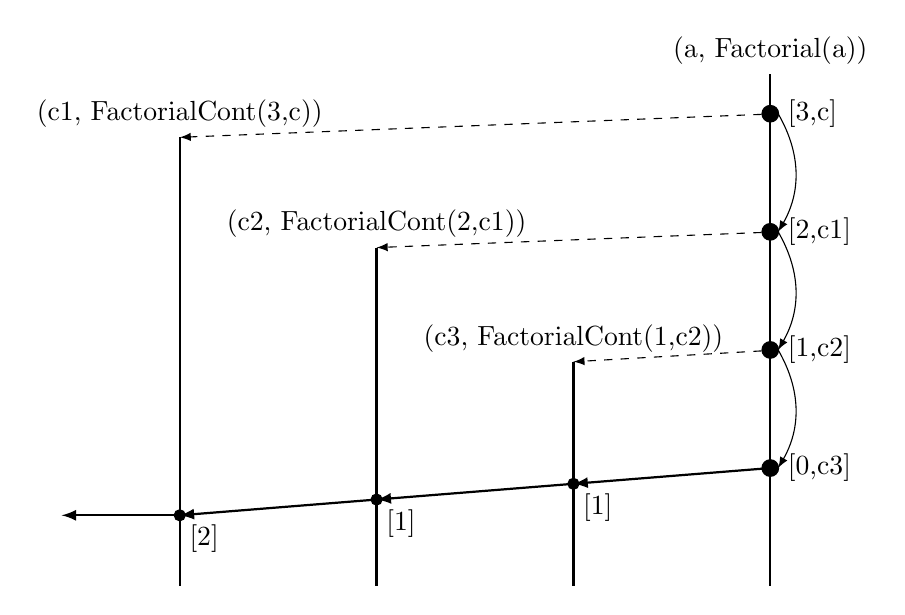
\begin{tikzpicture}
\draw[thick] (8,7) -- (8, 0.5);

\node[] (a1) at (8,7.3) {(a, Factorial(a))};

\node[align=center, right] (a1) at (8.1,6.5) {[3,c]};
\draw[fill] (8,6.5) circle (3pt);

\node[align=center, right] (a2) at (8.1,5) {[2,c1]};
\draw[fill] (8,5) circle (3pt);

\node[align=center, right] (a3) at (8.1,3.5) {[1,c2]};
\draw[fill] (8,3.5) circle (3pt);

\node[align=center, right] (a4) at (8.1,2) {[0,c3]};
\draw[fill] (8,2) circle (3pt);

\draw[-latex] (a1.west) to[bend left] (a2.west);
\draw[-latex] (a2.west) to[bend left] (a3.west);
\draw[-latex] (a3.west) to[bend left] (a4.west);

\node[] (d1) at (0.5,6.5) {(c1, FactorialCont(3,c))};
\draw[thick] (d1.south) -- (0.5, 0.5);

\node[] (c1) at (3,5.1) {(c2, FactorialCont(2,c1))};
\draw[thick] (c1.south) -- (3, 0.5);

\node[] (b1) at (5.5,3.65) {(c3, FactorialCont(1,c2))};
\draw[thick] (b1.south) -- (5.5, 0.5);

\draw[fill] (5.5,1.8) circle (2pt);
\node[align=center, right] (b2) at (5.5,1.5) {[1]};

\draw[fill] (3,1.6) circle (2pt);
\node[align=center, right] (c2) at (3,1.3) {[1]};

\draw[fill] (0.5,1.4) circle (2pt);
\node[align=center, right] (d2) at (0.5,1.1) {[2]};

\draw[-latex, thick] (8,2)  -- (5.5,1.8);
\draw[-latex, thick] (5.5,1.8) -- (3,1.6);
\draw[-latex, thick] (3,1.6) -- (0.5,1.4);
\draw[-latex, thick] (0.5,1.4) -- (-1,1.4);

\draw[-latex, black, dashed] (a1.west) -- (d1.south);
\draw[-latex, black, dashed] (a2.west) -- (c1.south);
\draw[-latex, black, dashed] (a3.west) -- (b1.south);

\end{tikzpicture}
\caption{El diagrama ilustra el cálculo del factorial de 3, todo el resultado es
enviado al actor \textit{c}. Las lineas en punto indican la creación de un actor.}
\label{fig:factorial}
\end{figure}

Otro ejemplo que podemos encontrar en \cite{Agha:1986:AMC:7929} es el de una pila,
que está representada con una lista enlazada cada nodo de esta lista es un actor. 

\begin{lstlisting}[language=sal, style=simple]
def node(content, link)
  [ case operation of
        pop : (customer)
        push : (new-content)
    end case ]
  if operation = pop then
    become link
    send content to customer
  enf if
  if operation = push then
    let P = new node(content, link)
      in become new node(new-content, P) 
  end if
end def

def Main() 
  let stack = new node(10, Nil)
    in send [push, 20] to stack ||
       send [push, 30] to stack
  end
end
\end{lstlisting}

El comportamiento $node$ recibe dos valores al momento de creación el contenido a guardar y la referencia al siguiente nodo en la red. \\
Cuando $operation$ es de tipo $push$, crea un nuevo $node$ que sera el nodo que quedará segundo en la red, 
tomando los valores que anteriormente tenía la cabeza. Por otra parte, el comportamiento de reemplazo para el actor actual tendrá 
como contenido el valor recién recibido y como $link$ al actor recién creado, de esta manera quedará primero en la red el valor recibido. \\
Cuando $operation$ es de tipo $pop$, se envía el valor que contiene el nodo a la dirección recibida en $customer$ y el comportamiento 
de reemplazo es $become\ link$, básicamente reenviá todos los mensajes que recibe en su buzón a $link$. \\
Puede observarse en el ejemplo, que el primer nodo creado tiene como valor $Nil$, esto es simplemente una referencia nula. 

\section{Un modelo en CSP}
Para empezar a describir como se modeló en \CSP, primero es importante hacer
referencia a que se utilizó \CSPm \cite{fdr}, que combina los operadores de \CSP\ 
originalmente propuesto por Hoare\cite{Hoare:1978:CSP:359576.359585}, y un lenguaje funcional. \\
En el proceso de traducción de \SAL\ a \CSPm, fue necesario construir un pequeño
\textit{runtime} para emular como los actores corren. Recordemos que la
naturaleza de \CSP\ es sincrónica y los actores no lo son. \\
Fue necesario concretamente desacoplar la creación de nuevos actores, y el proceso de comunicaciones. 

\subsection{Estructuras de apoyo}

\subsubsection{Enteros pequeños}

Para evitar la explosión de estados que causa utilizar todo el rango de enteros 64-bits, se generó una
una representación propia para reducir está explosión de estados. El valor de $MAX\_INT$ es el entero mas grande que se quisiera representar.

\begin{align*}
datatype\ SmallInt =&\ SI.\{0 \ldots MAX\_INT\} | Overflow \\
\\
add(SI.a, SI.b)\ =&\ let\ sum\ = a + b \\
&within\ if\ sum <= MAX\_INT\ then\ SI.sum\ else\ Overflow  \\
%
sub(SI.a, SI.b) =&\ let\ sub\ =\ a - b \\
& within\ if\ sub >= 0\ then\ SI.sub\ else\ Overflow \\
%
mult(SI.a, SI.b) =&\ let\ mult\ = a * b \\
& within\ if\ mult <= MAX\_INT\ then\ SI.mult\ else\ Overflow \\
eq(SI.a, SI.b)\ =&\ a == b \\
eq(\_, \_)\ =&\ false
\end{align*}


\subsubsection{Identificadores de actores}

Esta construcción nombra cada uno de los actores que van ser utilizados, también
guarda la cantidad de actores de un tipo dado. \\
Para la definición usa tipos algebraicos similares a los de Haskell soportados por \CSPm.

\begin{figure}[H]
\begin{align*}
  datatype\ ActorID &= ACTOR_1.\{1 \ldots N_1\} | \\
  & ACTOR_2.\{1, \ldots ,N_2\} | \\
  & ACTOR_k.\{1, \ldots, N_k\} | \\
  & Main.\{1\}
\end{align*}
\end{figure}

Ya que no existe en \CSP\ el concepto de instancia es necesario contar con todos los 
procesos que van a ser parte de la red definidos desde el principio, concretamente 
el valor que está entre llaves corresponde a la cantidad de elementos de este
tipo que van a ser necesarios. 

\subsubsection{Valores primitivos}

Representaremos las cadenas de caracteres utilizando $Atoms$, estas cadenas son inmutables y no existe ninguna operación sobre ellas.

\[
  datatype\ Atoms = ATOM_1 | ATOM_2 | \ldots | ATOM_n
\]

Finalmente, $VALUE$ es un tipo de datos que nos permite tener cierta flexibilidad al momento de enviar mensajes o crear actores.

\[
  datatype\ VALUE = ACTOR.ActorID | INT.SmallInt | ATOM.Atoms | None
\]

\subsection{Buzón}

Recodemos que la naturaleza de \CSP es sincronica y los actores no lo son para esto necesitamos desacoplar el envío de mensajes de la recepción. Para esto utilizamos una estructura intermedia que actúa de \textit{buzón}, y dos canales que sirven para comunicarse con ella.

\[
channel\ CommSend:ActorID.(VALUE, VALUE)\\
channel\ CommRecv:ActorID.(VALUE, VALUE)
\]

Un \textit{buzón} puede guardar más de una comunicación en su interior. Esto introduce un tipo de no determinismo ya que un actor puede sincronizar con cualquiera de las comunicaciones disponibles en su \textit{buzón}.\\
El comportamiento del proceso buzón depende de su estado, si no tiene ningún mensaje, si tiene algunos mensajes, o si está completo. Podríamos modelar un buzón que no tenga una cota superior, pero tendríamos problemas de explosión de estados.

\begin{itemize}
\item Si no tiene ningún mensaje, solo sincroniza mensajes por el canal $CommSend$.
\item Si tiene algunos mensajes, por los canales $CommSend$ y $CommRecv$.
\item Si está completo, solo por el canal $CommRecv$.
\end{itemize}

Puede que los nombre de los canales suenen poco intuitivos, es importante notar que provienen de la acciones vista desde los actores.

\begin{description}
\item [CommSend] Canal utilizado para comunicar desde cualquier actor hacia el buzón.
\item [CommRecv] Canal utilizado para comunicar del buzón hacia el actor asociado.
\end{description}

\begin{align*}
mailbox(i, \nil) =& CommSend?i.x \then mailbox(i, \trace{x}) \\
mailbox(i, \trace{x}) =& \\
CommRecv!i.x & \then mailbox(i, \nil) \Extchoice CommSend?i.y \then mailbox(i, \trace{x, y}) \\
mailbox(i, \trace{x, y}) =& \\
CommRecv!i.x & \then mailbox(i,\trace{y}) \Extchoice CommRecv!i.y \then mailbox(i, \trace{x}) 
\end{align*}

Por cada actor en la red, existe un \textit{buzón} con el mismo \textbf{ActorID}
asociado. \\ 
Un actor se bloquea esperando en $CommRecv$, cuando una nueva comunicación está
dispuesta a ser sincronizada, desde el \textit{buzón} hacia el actor esta es procesada.

\[
mailboxes  = \Interleave_{actor : \{| ActorID |\} } mailbox(actor, \nil) 
\]

$mailboxes$ representa todos los buzones puestos en paralelo utilizando el
operador \textit{Interleave}. Como no existe comunicación entre buzones,
siempre la comunicación es desde un actor hacia un buzón el operador
de \textit{Interleave} \cite[Cap. 2, p.~65]{Roscoe:1997:TPC:550448}. 

\begin{figure}[H] \label{ActorID}
\[
datatype\ ActorID = ACTOR_1.\{1, 2, 3\} | ACTOR_2.\{1, 2\} | Main.\{1\} \\
\\
\{| ActorID |\} \equiv \{ACTOR_1.1, ACTOR_1.2, ACTOR_2.3, ACTOR_2.1,  ACTOR_2.2, MAIN.1 \} \\
\\
\{| ACTOR_2 |\} \equiv \{ ACTOR_2.1, ACTOR_2.2 \}
\]
\caption{Ejemplo de notación} 
\end{figure}

\subsection{Crear nuevos actores}

Antes de empezar, un ejemplo para entender como funciona un aspecto fundamental
de los canales de \CSPm. 

\[
V = \{1,2,3\} \\
channel C:V.V \\
P1 = C?x!2 \then \Stop \\
P2 = C!1?y \then \Stop \\
SYSTEM = P1 \Parallel P2
\]

Del ejemplo anterior podemos ver que el canal \textbf{C} genera el alfabeto de
comunicación $\{ C.1.1, C.1.2, C.1.3, C.2.1, C.2.2, C.2.3, C.3.1, C.3.2, C.3.3 \}$.
En $P1$ tenemos la variable libre $x$ y en $P2$ tenemos la variable libre $y$,
es simple notar que al utilizar \textbf{`?'} podemos introducir el uso de una
variable libre y no así cuando utilizamos \textbf{`!'}.
Esto genera la sensación de poder enviar un mensaje utilizando \textbf{!} y
recibirlo usando \textbf{?}\cite[chap.~1,p.~27]{Roscoe:1997:TPC:550448}. 

Recordemos que en \CSP\ no existe el concepto de instancia, y debemos
tener definida la red de procesos desde el comienzo. Para resolver este problema, 
se presentan tres abstracciones.

La primera, es un conjunto de canales $CreateAsk$ y $Create$ el primero es utilizando
por quien está queriendo crear un nuevo actor y el otro por el actor que está por 
iniciar.

\[
channel\ CreateAsk:ActorID.(VALUE, VALUE)\\
channel\ Create:ActorID.(VALUE, VALUE)
\]

La segunda abstracción es un preámbulo que ocurre antes de un comportamiento, quien dota a este de 
los parámetros \textit{acquaiantence-list} y al mismo tiempo el otorga al actor su identificador 
único de buzón. Esto se comporta como una especie de maquina de actores.

\begin{align}
actors\_machine_k = \Interleave_{ id : \{| ACTOR_k |\} } & Create!id?(p1, p2) \then \\
&comportamiento_k(id, p1, p2)
\end{align}

En realidad, la creación es algo ficticio ya que tenemos una red de procesos \CSP esperando al 
evento $Create$ para arrancar con el comportamiento definido. \\
El conjunto definido por $ACTOR_k$ es equivalente a los elementos definidos  en $ActorID$, 
esto se puede ver en el ejemplo \ref{ActorID}. \\
Por esto es que decimos que no solo define el nombre, sino que al mismo tiempo está
estableciendo cuantos actores del tipo $ACTOR_k$ vamos a tener.
Siguiendo con esta idea, $actors_machine_k$, representa todos los actores 
que van ser iniciados en paralelo utilizando el operador de \textit{Interleave}.
Una vez sincronizado en el mensaje $Create$, se ejecuta el comportamiento que obtiene
el identificador del buzón y los parámetros recibidos.

La tercer abstracción es un proceso que conecta esto dos mensajes. 
 
\[
create(actorId) = CreateAsk!actorId?m \then Create.actorId!m \then STOP \\
creates = \Interleave_{actor : ActorID} create(actor)
\]

Como puede observarse, tenemos tantos procesos en paralelo como $ActorID$ existan, 
tal como muestra el ejemplo en \ref{ActorID}. \\
Tal vez esta abstracción podría haber sido omitida, pero juega un papel fundamental
en la construcción total del sistema, esto tiene que ver con en \CSP\ se puede elegir los 
eventos \cite[chap.~2,p.~55]{Roscoe:1997:TPC:550448} que se van a sincronizar, cuando 
veamos como compone todo el sistema esta idea quedará mas clara.


\subsection{Definición de comportamientos}
La idea de comportamiento fue introducida en la sección \ref{basicos:comportamientos}, 
podemos pensar a un comportamiento como una función que procesa una comunicación y tiene como salida,
nuevas comunicaciones, nuevos actores y el comportamiento de reemplazo para el
actor que esta procesando la comunicación.

\begin{align*}
&CommSend.actor_{buzon}!(p_1, p_2) & (Enviar\ Comunicaciones) \\ 
&CreateAsk!Actor_m.pid?(p_1, p_2) & (Crear\ nuevos\ actores)\\
&actor_{running}(self, p_1, p_2)  & (Comportamiento\ de\ reemplazo)
\end{align*}


\begin{description}
\item [Enviar Comunicaciones] En este caso le enviaremos al actor con buzón $actor_{buzon}$ la tupla $(p_1, p_2)$. 
\item [Crear nuevos actores] Obtendríamos mediante $Actor_m.pid$ el identificador de buzón del actor creado, y le enviaríamos los parámetros $(p_1, p_2)$ como \textit{acquaiantence-list}.
\item [Comportamiento de reemplazo] En este caso el comportamiento sería $actor_{running}$, de no contar con uno sería simplemente \Stop.
\end{description}


\subsection{Ejemplo: cálculo de factorial en CSPm}
Se utilizará en esencia el mismo ejemplo del factorial antes visto en sal \SAL,
está compuesto por dos comportamientos $Factorial$ y $FactorialWorker$.

\subsubsection*{Comportamiento de Factorial}

\[
factorial = Create.Factorial.1?(None, None) \then factorial_{running}(Factorial.1) 
\]

En el caso de la formula anterior, espera a sincronizar con un mensaje de
creación. Esto no solamente simula la creación, sino que al mismo tiempo se
asigna el buzón con nombre $Factorial.1$ al actor que está corriendo. Dentro de
la definición del comportamiento hace referencia a $self$ como nombre de
su propio buzón.

Notar que en este caso solo se necesita un actor de tipo $Factorial$.

\[
factorial_{running}(self) = CommRecv?self.(ACTOR.mailboxClient, INT.k) \then     \\
\textbf{if} (eq(k,SI.0)) \\
\quad  then \\
\quad \quad CommSend!mailboxClient.(INT.SI.1, None) \then factorialRunning(self) \\
\quad \textbf{else} \\
\quad \quad \textbf{let} \\
\quad \quad \quad newK = sub(k, SI.1) \\
\quad \quad \textbf{within} \\
\quad \quad \quad CreateAsk?FactorialWorker.pid!(INT.k, ACTOR.mailboxClient) \then \\
\quad \quad \quad CommSend!self.(ACTOR.FactorialWorker.pid, INT.newK)  \then \\
\quad \quad \quad factorial_{running}(self)
\]

Cuando recibe un entero distinto de cero ejecuta dos acciones, crea un actor \textbf{FactorialWorker} 
y se envía un mensaje a si mismo para evaluar el factorial de \textbf{n - 1}.\\
En este caso el comportamiento de reemplazo para el buzón actual no cambia.

\subsubsection*{Comportamiento de FactorialWorker}

En el caso del comportamiento de \textbf{FactorialWorker} vamos a necesitar
mas de un actor de este tipo, puede verse a continuación la notación antes vista, para poner en
paralelo tantos procesos como elementos existan en el conjunto $\{|FactorialWorker|\}$.

\[
factorialWorker = \Interleave_{x : \{|FactorialWorker|\}} Create!x?(k, mailboxClient) \\ 
\quad \then factorialWorker_{running}(x, k, mailboxClient)
factorialWorker_{running}(self, INT.k, ACTOR.mailboxClient) = \\
CommRecv.self?(INT.n, None) \then \\
\quad \textbf{let} \\
\quad \quad val = mult(n, k) \\
\quad \textbf{within} \\
\quad \quad CommSend.mailboxClient!(INT.val, None) \then \\
\quad \Stop
\]

Este comportamiento es muy simple, en el momento de creación recibe dos
parámetros, un entero \textbf{k} y un dirección de un buzón, al momento de
recibir una comunicación, efectúa la multiplicación y se lo envía a
$mailboxClient$.
En este caso no cuenta con comportamiento de reemplazo, entonces termina con $\Stop$

\subsection{Ejemplo: Una pila en CSPm}

\begin{align*}
node & = \Interleave_{x : \{|Node|\}} & Create.actorId?(INT.content, ACTOR.link) \\ 
& \then node_{running}(actorId, content, link) \\
& & node_{running}(self, content, link) = \\
& \quad CommRecv.self?(ATOM.PUSH, INT.newContent) \then \\
& \quad CreateAsk?Node.newNode!(INT.content, ACTOR.link) \then \\
& \quad nodeRunning(self, newContent, Node.newNode)\\
& \Extchoice \\
& \quad CommRecv.self?(ATOM.POP, ACTOR.client) \then  \\
& \quad CommSend.client!(INT.content, None) \then  \\
& \quad fwd(self, link)\\
\end{align*}

\[
  fwd(in, out) = CommRecv.in?msg \then CommSend.out!msg \then fwd(in, out)
\]


\subsection{Ejemplo: Un una cola en SAL}

Introducir el código en sal, y explicar como funciona.
\subsection{Ejemplo: Un una cola en CSPm}

Introducir el código en CSPm equivalente y explicar las particularidades.

\subsection{Ejemplo: Un cliente-servidor de chat en SAL}

Introducir el código en sal, y explicar como funciona.

\subsection{Ejemplo: Un cliente-servidor de chat en CSPm}

Introducir el código en CSPm equivalente y explicar las particularidades.

\subsection{Mapeando de SAL a CSPm}

TODO: Definir \textbf{translateExp}

La clase \textbf{Cmnd} con elementos de tipo S está dada por:

\begin{verbatim}
S :== S_1 ; S_2 | if b then S_1 else S_2 | send [e1, .., e_i] to a | become new
E(e_1, .. ,e_i) | let a_1 = new E_1(e_1,..,e_i) and ... a_j = new
E_1(e_1,..,e_i) { S } 
\end{verbatim}

definimos la funcion \textbf{translateCmd} de la siguiente forma:

\begin{verbatim}
translateCmd (S_1 S_2) = translateCmd(S_1) -> translateCmd(S_2)
\end{verbatim}


\begin{verbatim}
translateCmd(if b then S_1 else S_2) = 
   if (translateExp(b)) then
       translateCmd(S_1) else 
       translateCmd(S_2)
\end{verbatim}

\begin{verbatim}
translateCmd(send[e_1, ..., e_i] to a) = CommSend.a.
         (translateExp(e_1), ..., 
          translateExp(e_i)) 
\end{verbatim}

\begin{verbatim}
translateCmd(become new Beh(e_1, ..., e_n)) = runningBeh(self, e_1, ..., e_n)
\end{verbatim}

newEnv es el resultado de agregar a el entorno de las variables de mailbox $a_1
= E_1.pid_1$ .. $a_n = E_n.pid_n$
\begin{verbatim}
translateCmd(let a_1 = new E_1(e_1, ..., e_j) and 
         ... and a_n = new E_N(e_1, ..., e_j) { S } = 

CreateAsk?E_1.pid_1!(translateExp(e_1), ...,translateExp(e_j)) ->
CreateAsk?E_N.pid_n!(translateExp(e_1), ...,translateExp(e_j)) ->
translateCmd(S, newEnv)
\end{verbatim}


La clase \textbf{Beha} con elementos de tipo S está dada por:

\begin{verbatim}
def behName(a_1 .. a_i)[n_1 ... n_j]
  S
end def
\end{verbatim}

Tendria como equivalente en CSP:

\begin{verbatim}

behName = ||| actorId : {|BehName|} @ Create.actorId?(a_1, ..., a_i) ->
behNameRunning(actorId, a_1, .., a_n)

behNameRunning(self, a_1, .., a_n) = CommRecv.self(n_1 ... n_j) -> translateCmd(S)

\end{verbatim}

--- Agregar case? ---

\bibliography{references}{}
\bibliographystyle{plain}
\end{document}



